\documentclass{beamer}

\usepackage[french]{babel}
\usepackage[T1]{fontenc}
\usepackage[utf8]{inputenc}

\usetheme{Warsaw}
\useoutertheme{infolines}

\usepackage{amsmath}
\usepackage{amssymb}
\usepackage{amsthm}
\usepackage{stmaryrd}

\usepackage{listings}
\usepackage{color}

\definecolor{mygreen}{rgb}{0,0.6,0}
\definecolor{mygray}{rgb}{0.5,0.5,0.5}
\definecolor{mymauve}{rgb}{0.58,0,0.82}

\lstset{ %
  backgroundcolor=\color{white},   % choose the background color
  basicstyle=\footnotesize,        % size of fonts used for the code
  breaklines=true,                 % automatic line breaking only at whitespace
  captionpos=b,                    % sets the caption-position to bottom
  commentstyle=\color{mygreen},    % comment style
  escapeinside={\%*}{*)},          % if you want to add LaTeX within your code
  keywordstyle=\color{blue},       % keyword style
  stringstyle=\color{mymauve},     % string literal style
}

\usepackage[all]{xy}

%Les sous listes on des triangles
\setbeamertemplate{itemize item}[circle]
\setbeamertemplate{itemize subitem}[triangle]
%Les elements caché sont grisé
\beamertemplatetransparentcovered

\begin{document}

\title{Android - Les bonnes intentions}
\author{Jérémy S. Cochoy}
\institute{INRIA Paris-Saclay | jeremy.cochoy@u-psud.fr}
\date{Novembre 2015}


\begin{frame}
\titlepage
\end{frame}

\begin{frame}
\tableofcontents
\end{frame}

\begin{frame}
\frametitle{La documentation}

\begin{block}{Votre nouveau livre de chevet.}
\begin{center}
\emph{https://developer.android.com/guide/index.html}
\end{center}
\end{block}

\end{frame}

\section{GIT et GitHub}

\begin{frame}
\frametitle{GitHub}
\begin{center}

\includegraphics[scale=0.4]{github.jpg}
\end{center}
\end{frame}

\section{Intention}

\begin{frame}
\frametitle{Qu'est-ce qu'une intention?}

\begin{block}{Une \verb!Intent!}
Une \verb!Intent! est un objet qui représente un message, et permet de demander une action à un Composant.
\end{block}

\begin{block}{Les usages principaux :}
	\begin{itemize}
		\item Lancer une activité.
		\item Lancer un service.
		\item Délivrer un message.
	\end{itemize}
\end{block}
\end{frame}


\begin{frame}
\frametitle{Démarrer une activité}

\begin{block}{\verb!Activity!}
Une \verb!Activity! représente un écran dans une app. On peut lancer une activité en donnant un \verb!Intent! à \verb!startActivity()!. L'intention décrit l'activité et lui fournit les données.
\end{block}

\begin{block}{Avec résultat}
Si l'activité doit fournir un résultat, on dispose de \verb!startActivityForResult()! et de \verb!onActivityResult()!.
\end{block}
\end{frame}

\begin{frame}
\frametitle{Démarrer un service}

\begin{block}{Un service effectue des actions en arrière plan, sans interface.}

\begin{itemize}
\item One time operation : Donner un Intent à \verb!startService()!.
\item Si le service a une interface client-serveur, on dispose de \verb!bindService()!.
\end{itemize}
\end{block}
\end{frame}

\begin{frame}
\frametitle{Délivrer un message}

\begin{block}{Broadcast}
Un broadcast est un message que n'importe quelle application peut recevoir.
\end{block}

\begin{block}{Délivrer un message}
Donner un \verb!Intent! à \verb!sendBroadcast()! ou \verb!sendOrderedBroadcast()!.
\end{block}
\end{frame}

\begin{frame}
\begin{block}{Deux types d'Intent :}
\begin{itemize}
\item Explicite : Contient le nom du composant explicite.
\item Implicite : Décrit une action à effectuer (url, localisation, ...).
\end{itemize}

\end{block}
\end{frame}

\begin{frame}
\frametitle{Filtres}
\begin{center}
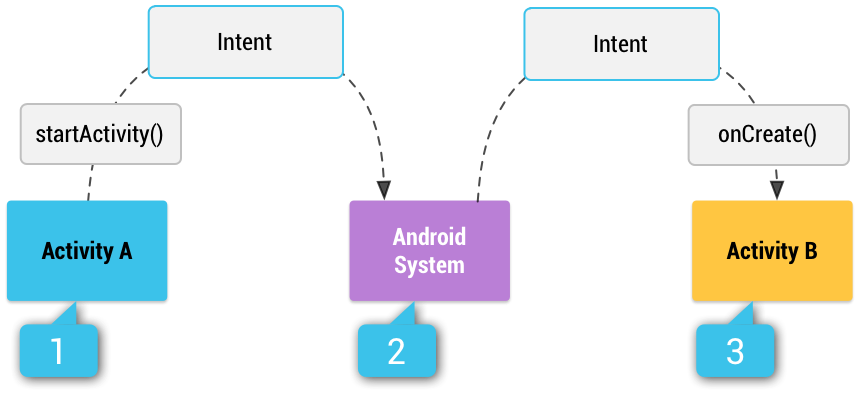
\includegraphics[scale=0.3]{intent-filters2.png}
\end{center}
\end{frame}

\begin{frame}[fragile]
\frametitle{Exemple de filtre}
\begin{block}{Filtrer le partage d'images}
\lstset{language=XML}
\begin{lstlisting}
<activity android:name="ShareActivity">
 <intent-filter>
  <action android:name="android.intent.action.SEND"/>
  <category android:name="android.intent.category.DEFAULT"/>
  <data android:mimeType="image/*"/>
 </intent-filter>
</activity>
\end{lstlisting}
\end{block}
\end{frame}

\begin{frame}
\frametitle{Construire une intention}
\begin{block}{Une intention contient les informations suivantes :}
\begin{itemize}
\item Nom du composant
\item Action
\item Data
\item Category
\item Extras
\end{itemize}
\end{block}
\end{frame}

\begin{frame}
\frametitle{Nom du composant}
\begin{block}{Le nom du composant à lancer}
Nécessaire pour une intention explicite.
\end{block}
\begin{block}{}
Un \verb!Service! doit toujours être lancer explicitement.
\end{block}
Le champ de l'\verb!Intent! est un objet \verb!ComponentName! qui contient un chemin complet vers le nom de la classe. Par exemple : \emph{com.example.ExampleActivity}. La valeur peut être fixée avec \verb!setComponent()!, \verb!setClass()!, \verb!setClassName()!, ou le constructeur de l'\verb!Intent!.

\end{frame}

\begin{frame}
\frametitle{Action}
Une chaîne qui spécifie le type d'action à effectuer.

\begin{block}{Quelques actions classiques}
\begin{itemize}
\item \verb!ACTION\_VIEW! Avec \verb!startActivity()! pour afficher une information (Photo, localisation...)
\item \verb!ACTION\_SEEND! Avec \verb!startActivity()! , pour "partager" (share).
\item \verb!ACTION\_EDIT! Fournit un document à éditer.
\item \verb!ACTION\_PICK! Sélectionne un fichier / image / etc...
\end{itemize}
\end{block}
\end{frame}

\begin{frame}
\frametitle{Data}
L'objet \verb!Uri! qui contient une référence / lien vers les données à transmettre.

\medskip

Il est bon de préciser le type.

\medskip

Les méthodes \verb!setData()!, \verb!setType()! sont exclusives, mais \verb!setDataAndType()! permet de spécifier les deux.
\end{frame}

\begin{frame}
\frametitle{Extra}
Permet de passer des données sous la forme clef-valeur.

\medskip

Via la méthode \verb!putExtra()!, ou un \verb!Bundle! avec \verb!putExtras()!.

\begin{block}{Exemple :}
Dans un ACTION\_SEND, on peut vouloir ajouter les valeurs EXTRA\_EMAIL et EXTRA\_SUBJECT pour envoyer un e-mail.
\end{block}

\end{frame}

\begin{frame}
\frametitle{Catégories}
\begin{itemize}

\item Permet d’être plus précis sur quelles activités sont concernées.

\item La CATEGORY\_DEFAULT convient à la plupart des usages.

\item Par exemple, CATEGORY\_BROWSABLE spécifie que l'élément transmit peut être ouvert par un navigateur web.
\end{itemize}
\end{frame}

\begin{frame}[fragile]
\frametitle{Exemple explicite :}
\lstset{language=java}

\begin{block}{Explicit intent}
\begin{lstlisting}
// Executed in an Activity, so 'this' is the Context
// The fileUrl is a string URL, such as "http://www.example.com/image.png"
Intent downloadIntent = new Intent(this, DownloadService.class);
// DownloadService is the name of the app.
downloadIntent.setData(Uri.parse(fileUrl));
startService(downloadIntent);
\end{lstlisting}
\end{block}
\end{frame}


\begin{frame}[fragile]
\frametitle{Exemple implicite :}
\lstset{language=java}

\begin{block}{Implicit intent}
\begin{lstlisting}
// Create the text message with a string
Intent sendIntent = new Intent();
sendIntent.setAction(Intent.ACTION_SEND);
sendIntent.putExtra(Intent.EXTRA_TEXT, textMessage);
sendIntent.setType("text/plain");

// Verify that the intent will resolve to an activity
if (sendIntent.resolveActivity(getPackageManager()) != null) {
    startActivity(sendIntent);
}
\end{lstlisting}
\end{block}
\end{frame}

\section{Activités}

\begin{frame}

\frametitle{Cycle de vie d'une activité}

\begin{center}
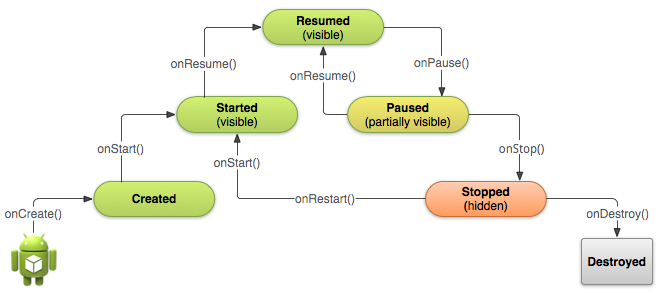
\includegraphics[scale=0.5]{basic-lifecycle.png}
\end{center}
\end{frame}

\begin{frame}
\begin{center}
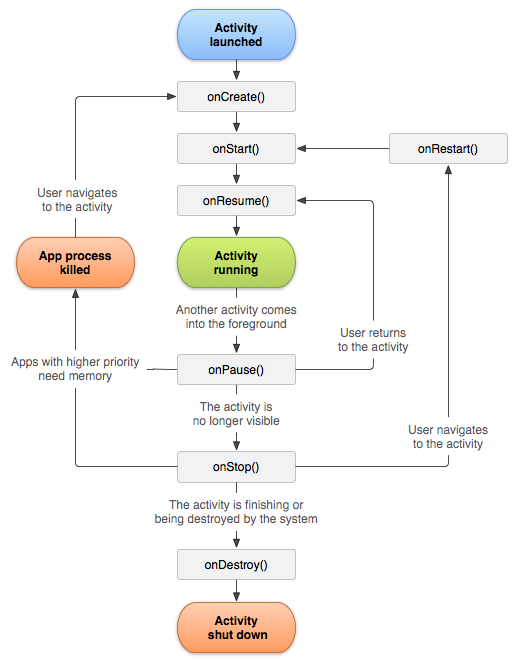
\includegraphics[scale=0.3]{activity_lifecycle.png}
\end{center}

\end{frame}
\lstset{language=java}
\begin{frame}[fragile]
\begin{lstlisting}
public class ExampleActivity extends Activity {
    @Override
    public void onCreate(Bundle savedInstanceState) {
        super.onCreate(savedInstanceState);
        // The activity is being created.
    }
    @Override
    protected void onStart() {
        super.onStart();
        // The activity is about to become visible.
    }
    @Override
    protected void onResume() {
        super.onResume();
        // The activity has become visible (it is now "resumed").
    }
\end{lstlisting}
\end{frame}
\begin{frame}[fragile]
\begin{lstlisting}
    @Override
    protected void onPause() {
        super.onPause();
        // Another activity is taking focus (this activity is about to be "paused").
    }
    @Override
    protected void onStop() {
        super.onStop();
        // The activity is no longer visible (it is now "stopped")
    }
    @Override
    protected void onDestroy() {
        super.onDestroy();
        // The activity is about to be destroyed.
    }
}
\end{lstlisting}

\end{frame}
\section{Conclusion}

\begin{frame}
\begin{center}
Pour me contacter : jeremy.cochoy@u-psud.fr, merci et à bientôt.

\medskip
\medskip
\medskip
\medskip


\includegraphics[scale=0.18]{android.jpg}
\end{center}
\end{frame}

\end{document}
